\newpage
\section{Introdução}
\label{sc:Introducao_}


{
\onehalfspacing
O agronegócio no Brasil possui caráter de grande envergadura para toda a economia do país. Somente em maio de 2017, as exportações atingiram US\$ 9,68 bilhões, valor que corresponde a aproximados 13\% de aumento em referência ao mesmo período do ano anterior. Somente o valor desse superávit comercial causou um aumento de 790 milhões de dólares, demonstrando que esse setor possui alta taxa de crescimento. Dentre parte das exportações, está contida o setor de carnes, com arrecadação em 2017, de 1,22 bilhão de dólares. (SANTANDER, 2017)
}

{
Todavia, mesmo com notório crescimento, muitos fazendeiros passam por inúmeras dificuldades para acompanhar seu gado, devido a sua ausência por problemas do cotidiano que simplesmente impedem a presença diária do fazendeiro para o acompanhamento. Devido a isso, surgem ocasiões que geram transtornos e podem gerar prejuízo, tais como perder vacas por terem fugido da propriedade, por ficarem atoladas, ou mesmo perder muito tempo procurando o gado em um determinado local sendo que o mesmo pode estar no outro extremo da região. Levando em consideração tais problemas, propõem-se formas de monitorar o gado à distância, para um melhor gerenciamento por parte dos fazendeiros.
}

{
A solução proposta por todo o projeto\footnote{O projeto completo constitui-se de duas partes separadas, que serão desenvolvidas em paralelo. A primeira parte é a que constitui o código fonte de todo o sistema de monitoramento e gerenciamento. A segunda parte constitui-se do Hardware envolvido nos nós da rede, nos estudos referentes aos modelos de bateria e nos diferentes modos de operação envolvidos no estudo do consumo do circuito.} visa realizar o monitoramento e gerenciamento dos animais à distância, usando de tecnologias especificas, tais como o IoT - Internet of Things, cuja tradução direta é “Internet das Coisas”, microchips inteligentes como o ESP8266, ESP32, ATtiny13 dentre outros e protocolos de comunicações e de gerenciamento de sinais, como o Wi-Fi, Bluetooth Low Energy, RSSI e MQTT.
}

{
Os principais preceitos do IOT se baseiam na ligação entre alguma “coisa” física ao meio das comunicações de rede dinâmica e global, portando, dessa maneira, a capacidade de configurar de forma inteligente ou interagir com o objeto físico em questão. Para tal interfaceamento, utilizam-se sistemas eletrônicos pré-programados conectados em alguma rede, bem como na rede global. Esta comunicação pode se dar pelo uso do Wi-Fi ou do Bluetooth.
}

{
Os chips inteligentes utilizados detêm a função de controlarem a comunicação entre si, utilizando protocolos de comunicações específicos, e gerenciar os dados colhidos. Para isso, serão pré-programados afim de cumprirem com suas respectivas funções.
}

{
Para o amplo emprego dessas tecnologias, é preciso viabilizar algumas características fundamentais no sistema, sendo estes o tamanho do projeto final, o custo e a autonomia, que é definida como o período máximo que o circuito poderá ser mantido em constante funcionamento sem apresentar falhas. Para se alcançar um bom valor, foram empregadas as mais recentes formas de tecnologia de baixo consumo disponíveis no mercado, que consistiu no emprego de Microcontroladores específicos e de modos de comunicação aplicados ao baixo consumo, além do aprimoramento de técnicas justapostas que relacionam dois ou mais modos de operação para uma combinação satisfatória de baixo consumo.
}

{
Um desafio no que diz respeito ao emprego desse sistema está justamente em cumprir com uma boa viabilidade o tamanho e o custo final do sistema eletrônico, sem que se perca a autonomia necessária para o funcionamento do código fonte\footnote{O código fonte resume-se nas operações pré-programadas que o circuito eletrônico fará atuando no meio físico.}, que será desenvolvido paralelamente pela UFSJ – Universidade Federal de São João Del-Rei. Será considerado um tamanho que caiba em uma etiqueta utilizada pelos fazendeiros para a identificação de cada animal, como mostrado na figura \ref{fig:modelo_etiqueta}, a qual é presa em suas respectivas orelhas. Seguidamente, será analisado o custo do protótipo, a qual recorre da compra de basicamente dois principais componentes: o processador utilizado e a bateria escolhida para alimentar o circuito.
}

\begin{figure}[htb]
    \centering
    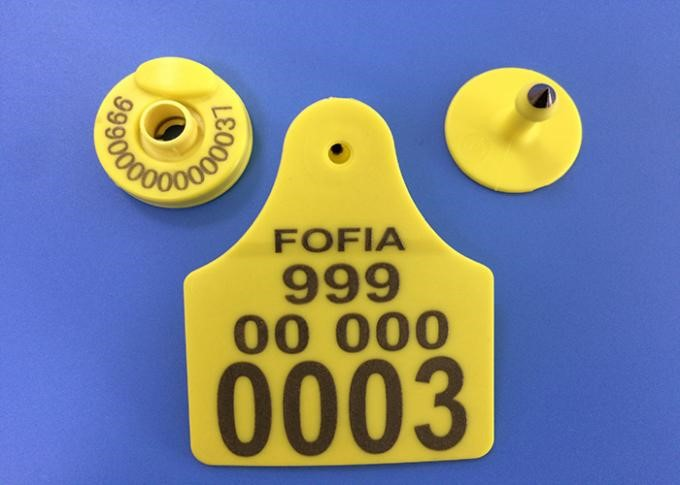
\includegraphics[scale = 0.4]{img/Modelo_de_etiqueta.jpg}
    \caption{Modelo de etiqueta.}
    \label{fig:modelo_etiqueta}
\end{figure}

{
Levando-se esses problemas em consideração, os Microcontroladores escolhidos para a realização dos estudos foram os referentes à família ESP e a família ATtiny, sendo seus principais polos o ESP8266, o ESP32 e o ATtiny13A-PU. Todos foram escolhidos por apresentarem alto desempenho em eficiência energética. Ademais, esses Microcontroladores apresentam a portabilidade de modelos de comunicação distintos, de modo que o ESP8266 possa utilizar o Wi-Fi, o ESP32 possa utilizar o BLE - Bluetooth Low Energy, e, por fim, o ATtiny13 possui compatibilidade com módulos de rádio frequência, como o NRF24l01.
}

{
Com tais Microcontroladores, pode-se contornar o problema de custo e autonomia, visto que se apresentam de fácil acesso e apresentam tecnologias já inclusas de baixo consumo. Além disso, apresentam boa compatibilidade com o tamanho total do projeto, facilitando a instalação na etiqueta.
}

{
Após a escolha dos referidos Microcontroladores, foram realizadas inúmeras análises de diversos modelos de baterias, com a finalidade de se obter o modelo que melhor atende às necessidades de tamanho, custo e capacidade energética, para acréscimo da autonomia. 
}

{
Mais especificamente, nesse projeto será montado um protótipo operacional de um dos nós da rede de integração de monitoramento do gado, utilizando um dos dois chips ESP, com o intuito de chegar a possíveis soluções para o projeto. Nas Figuras \ref{fig:prototipo_tamanho_esp32} e \ref{fig:prototipo_tamanho_esp8266}, apresentam-se as versões que servirão como base para os futuros protótipos, levando em consideração os modelos de bateria da mesma proporção, além dos pequenos componentes externos necessários para o funcionamento do circuito.
}

\begin{figure}[htp]
    \centering
    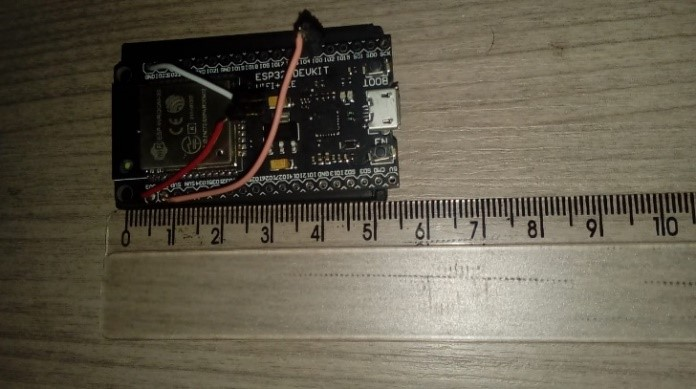
\includegraphics[scale = 0.9]{img/prototipo_ESP32_tamanho.jpg}
    \caption{Modelo de protótipo utilizando o ESP32}
    \label{fig:prototipo_tamanho_esp32}
\end{figure}

\begin{figure}[htp]
    \centering
    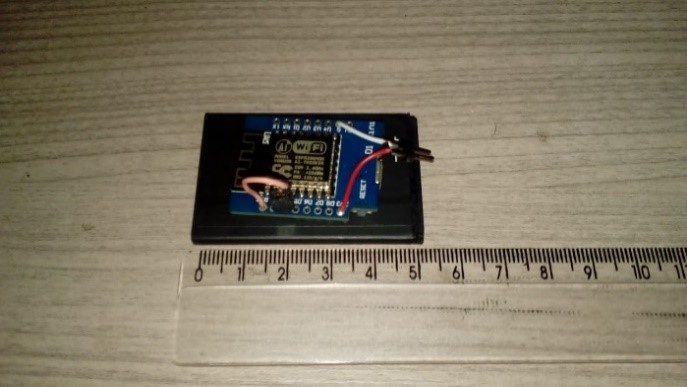
\includegraphics[scale = 0.9]{img/prototipo_ESP8266_tamanho.jpg}
    \caption{Modelo de protótipo utilizando o ESP8266}
    \label{fig:prototipo_tamanho_esp8266}
\end{figure}



